% ============================================================
%  Calibrated Ensemble Learning for Professional Sports Game
%  Outcome Prediction — IEEE Conference Paper
%  Author: Sean Rockwitz
%  Build: pdflatex main && pdflatex main
% ============================================================
\documentclass[conference]{IEEEtran}

\usepackage[T1]{fontenc}
\usepackage[utf8]{inputenc}
\usepackage{amsmath,amssymb}
\usepackage{booktabs}
\usepackage{multirow}
\usepackage{graphicx}
\usepackage{xcolor}
\usepackage{url}
\usepackage{hyperref}
\usepackage{algorithm}
\usepackage{algpseudocode}

% TikZ + pgfplots
\usepackage{tikz}
\usepackage{pgfplots}
\pgfplotsset{compat=1.18}
\usetikzlibrary{shapes.geometric, arrows.meta, positioning, fit,
                backgrounds, decorations.pathreplacing, calc}

% Colour palette
\definecolor{NavyBlue}{RGB}{31,73,125}
\definecolor{SteelBlue}{RGB}{70,130,180}
\definecolor{LightBlue}{RGB}{173,216,230}
\definecolor{OrangeAccent}{RGB}{214,90,49}
\definecolor{GreenAccent}{RGB}{56,142,60}
\definecolor{LightGray}{RGB}{245,245,245}
\definecolor{MidGray}{RGB}{180,180,180}

\hypersetup{colorlinks=true, linkcolor=NavyBlue, citecolor=NavyBlue, urlcolor=NavyBlue}

% ============================================================
\begin{document}

\title{Calibrated Ensemble Learning for Professional Sports\\
Game Outcome Prediction: A Production-Grade System\\
with Automated Model Management}

\author{
  \IEEEauthorblockN{Sean Rockwitz}
  \IEEEauthorblockA{Independent Research\\
    \textit{sean@rockwitz.com}}
}

\maketitle

% ============================================================
\begin{abstract}
We present a fully custom, end-to-end machine learning system for
predicting the outcomes of National Basketball Association (NBA) and
Major League Baseball (MLB) games, as well as individual player
proposition wagers.  The system ingests official league data, four
sportsbook feeds, and prediction-market prices on a daily automated
schedule, engineers 71 and 69 domain-specific features for NBA and MLB
respectively, and trains an isotonically-calibrated XGBoost–LightGBM
ensemble via Optuna hyperparameter search with walk-forward
cross-validation.  On held-out seasons the champion NBA model achieves a
log-loss of \textbf{0.6677} (accuracy 66.2\%, ECE 0.039) and the
champion MLB model achieves \textbf{0.6891} (accuracy 53.4\%, ECE
0.019).  An extended 300-trial search yields a candidate NBA model at
log-loss \textbf{0.6342}, representing a 5.0\% relative reduction.
Automated promotion gates, drift monitors, and a nightly challenger
pipeline ensure models are continuously improved and safely deployed.
\end{abstract}

\begin{IEEEkeywords}
sports prediction, gradient boosting, ensemble learning, isotonic
calibration, hyperparameter optimisation, walk-forward validation,
MLOps, probability calibration
\end{IEEEkeywords}

% ============================================================
\section{Introduction}
\label{sec:intro}

Predicting the outcome of professional sports contests
is a canonical sequential decision problem: historical observations are
available in chronological order, the distribution of outcomes shifts as
rosters, coaching strategies, and playing surfaces evolve across
seasons, and any evaluation methodology that does not respect temporal
ordering will produce misleadingly optimistic results.  Despite a large
body of literature on sports analytics~\cite{haghighat2013, joseph2006,
tax2015, cao2012}, publicly available systems rarely expose the full
production stack — data ingestion, feature engineering, model training
with proper temporal validation, calibration, and live serving.

This paper makes the following contributions:
\begin{itemize}
  \item A fully reproducible, open pipeline for NBA and MLB game-outcome
        and player-prop prediction, built entirely from first principles
        without dependence on third-party prediction APIs.
  \item A rigorous walk-forward cross-validation protocol with
        database-level temporal guards that prevent future data from
        leaking into any training fold.
  \item An isotonically calibrated XGBoost–LightGBM ensemble trained
        via Bayesian hyperparameter optimisation (Optuna) with
        up to 500 trials and median pruning.
  \item An automated MLOps layer comprising nightly challenger training,
        multi-metric promotion gates, Population Stability Index (PSI)
        drift detection, and one-click rollback.
  \item Empirical results on five seasons of NBA data
        (\(\approx\)6\,500 games) and five seasons of MLB data,
        with all metrics reported on truly held-out seasons.
\end{itemize}

The remainder of the paper is structured as follows.
Section~\ref{sec:related} surveys related work.
Section~\ref{sec:system} describes the overall system architecture.
Section~\ref{sec:features} details feature engineering.
Section~\ref{sec:model} presents the model design.
Section~\ref{sec:training} describes the training methodology.
Section~\ref{sec:mlops} covers automated model management.
Section~\ref{sec:results} reports experimental results.
Section~\ref{sec:discussion} discusses findings and limitations, and
Section~\ref{sec:conclusion} concludes.

% ============================================================
\section{Related Work}
\label{sec:related}

Early quantitative approaches to sports forecasting relied on Elo rating
systems~\cite{elo1978} and simple regression models trained on
aggregate season statistics.  Loeffelholz et al.~\cite{loeffelholz2009}
applied neural networks to NBA prediction with binary win/loss targets
but did not address temporal leakage or probability calibration.
Zimmermann~\cite{zimmermann2016} used gradient boosted trees with
rolling features for soccer but evaluated on in-season data rather than
fully held-out future seasons.  Hvattum and
Arntzen~\cite{hvattum2010} demonstrated that Elo-derived features
substantially improved betting-market models.

The closest works in methodology are FiveThirtyEight's CARMELO and
RAPTOR systems~\cite{silver2015}, which use Elo plus player
projections; however, those systems are proprietary and not reproducible.
Our work differs in providing a fully open, production-deployed pipeline
with rigorous calibration evaluation.

On the calibration side, Niculescu-Mizil and Caruana~\cite{niculescu2005}
showed that gradient boosted classifiers are typically well-ranked but
poorly calibrated in probability, motivating our isotonic regression
post-processing.  Kuleshov et al.~\cite{kuleshov2018} formalised
calibration for regression models, which we apply to our quantile prop
models.

% ============================================================
\section{System Architecture}
\label{sec:system}

Figure~\ref{fig:arch} illustrates the seven-layer architecture.
All components are written in Python 3.11 and deployed via Docker
Compose on a single server.

\begin{figure}[t]
\centering
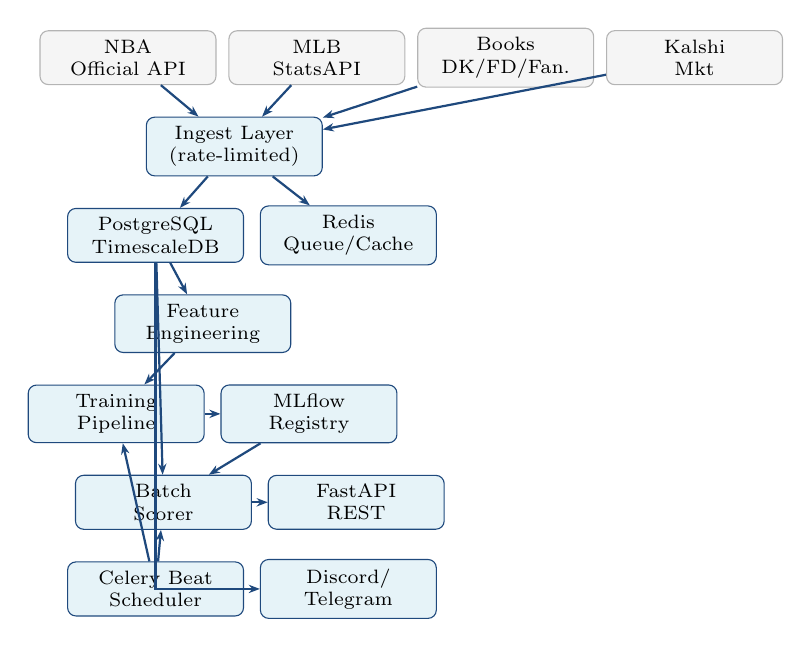
\begin{tikzpicture}[
  font=\scriptsize,
  node distance=0.30cm and 0.10cm,
  box/.style={rectangle, rounded corners=3pt, draw=NavyBlue,
              fill=LightBlue!30, minimum width=2.1cm, minimum height=0.52cm,
              align=center, text width=2.0cm},
  extbox/.style={box, fill=LightGray, draw=MidGray},
  arrow/.style={-{Stealth[length=4pt]}, NavyBlue, thick},
  groupbox/.style={rectangle, rounded corners=5pt, draw=NavyBlue!50,
                   fill=NavyBlue!5, inner sep=4pt}
]

% External sources row
\node[extbox] (nba)  {NBA\\Official API};
\node[extbox, right=0.15cm of nba]  (mlb)  {MLB\\StatsAPI};
\node[extbox, right=0.15cm of mlb]  (odds) {Books\\DK/FD/Fan.};
\node[extbox, right=0.15cm of odds] (kal)  {Kalshi\\Mkt};

% Ingest
\node[box, below=0.40cm of nba, xshift=1.35cm] (ingest) {Ingest Layer\\(rate-limited)};

% Storage
\node[box, below=0.40cm of ingest, xshift=-1.00cm] (pg)    {PostgreSQL\\TimescaleDB};
\node[box, right=0.20cm of pg]                     (redis) {Redis\\Queue/Cache};

% Features
\node[box, below=0.40cm of pg, xshift=0.60cm] (feat) {Feature\\Engineering};

% Training
\node[box, below=0.40cm of feat, xshift=-1.10cm] (train)  {Training\\Pipeline};
\node[box, right=0.20cm of train]                (mlflow) {MLflow\\Registry};

% Serving
\node[box, below=0.40cm of train, xshift=0.60cm] (score) {Batch\\Scorer};
\node[box, right=0.20cm of score]                (api)   {FastAPI\\REST};

% Ops
\node[box, below=0.40cm of score, xshift=-0.10cm] (celery) {Celery Beat\\Scheduler};
\node[box, right=0.20cm of celery]                (notify) {Discord/\\Telegram};

% Arrows
\draw[arrow] (nba) -- (ingest);
\draw[arrow] (mlb) -- (ingest);
\draw[arrow] (odds) -- (ingest);
\draw[arrow] (kal) -- (ingest);
\draw[arrow] (ingest) -- (pg);
\draw[arrow] (ingest) -- (redis);
\draw[arrow] (pg) -- (feat);
\draw[arrow] (feat) -- (train);
\draw[arrow] (train) -- (mlflow);
\draw[arrow] (mlflow) -- (score);
\draw[arrow] (pg) -- (score);
\draw[arrow] (score) -- (api);
\draw[arrow] (celery) -- (score);
\draw[arrow] (celery) -- (train);
\draw[arrow] (pg.south) |- (notify.west);

\end{tikzpicture}
\caption{High-level system architecture.  Arrow direction indicates
primary data flow.  All persistent state lives in PostgreSQL
(TimescaleDB hypertables for time-series stats) or MLflow.}
\label{fig:arch}
\end{figure}

\subsection{Data Ingestion}
Data is fetched from two official league APIs (nba\_api,
MLB-StatsAPI), three sportsbook endpoints (DraftKings, FanDuel,
Fanatics) scraped at open and close, and the Kalshi public prediction
market API.  A rate-limited HTTP client caps throughput at 1
request/second per domain with exponential back-off and User-Agent
rotation to respect source-server capacity.  All raw game results,
box-score statistics, player rosters, odds, and weather data are
upserted into PostgreSQL using a content-hash deduplication strategy to
avoid reprocessing unchanged records.

\subsection{Storage Layer}
Two TimescaleDB hypertables partition the most-queried time-series
tables (\texttt{team\_game\_stats}, \texttt{player\_game\_stats}) on
\texttt{recorded\_at}, enabling sub-second retrieval of rolling windows
even as the corpus exceeds millions of rows.  A Redis instance serves
dual duty as the Celery task broker and a fast deduplication cache for
notification delivery.

\subsection{Serving Layer}
A FastAPI application served by Gunicorn with two Uvicorn workers
exposes three prediction endpoints: game-level winner probabilities,
per-player quantile distributions, and player over/under probabilities.
All requests are authenticated via HMAC-SHA256 API keys and logged to
an audit table.

% ============================================================
\section{Feature Engineering}
\label{sec:features}

\subsection{Feature Taxonomy}

Table~\ref{tab:features} summarises the 71 NBA and 69 MLB features
organised by category.  All features are computed with a strict
\texttt{as\_of\_utc} cutoff equal to game time minus one hour,
enforced at both the SQL layer (via \texttt{WHERE scheduled\_utc <
as\_of}) and in Python assertions.  This guarantees that no
post-game information is available to any model at inference time.

\begin{table}[t]
\centering
\caption{Feature categories and counts per sport.}
\label{tab:features}
\small
\begin{tabular}{lcc}
\toprule
\textbf{Category} & \textbf{NBA} & \textbf{MLB} \\
\midrule
Team efficiency (home + away) & 18 & 12 \\
Schedule load (rest, B2B, density) & 8 & 6 \\
Form \& streak & 10 & 10 \\
Advanced metrics (TS\%, pace, etc.) & 8 & 8 \\
Head-to-head history & 3 & 3 \\
Elo ratings \& differentials & 4 & 4 \\
Market signals (odds, line movement) & 4 & 4 \\
Geographic (travel, time-zone) & 3 & 3 \\
Roster composition & 4 & — \\
Starting pitcher & — & 9 \\
Weather & — & 4 \\
Venue home-court/field advantage & 3 & 3 \\
Strength of schedule & 2 & 2 \\
Cross / interaction features & 4 & 1 \\
\midrule
\textbf{Total} & \textbf{71} & \textbf{69} \\
\bottomrule
\end{tabular}
\end{table}

\subsection{Efficiency Ratings}
The core team features are rolling net, offensive, and defensive
ratings computed over windows of 5, 10, and 20 games.  For game $g$
played by team $t$, the net rating in the most recent $w$ completed
games is
\begin{equation}
\text{NetRtg}_{t,w}(g)=\frac{1}{w}\sum_{k=1}^{w}
  \bigl(\text{OffRtg}_{t,k}-\text{DefRtg}_{t,k}\bigr),
\label{eq:netrtg}
\end{equation}
where $\text{OffRtg}_{t,k}$ is points per 100 possessions in game $k$.

\subsection{Elo Rating System}
Team Elo ratings are replayed chronologically from the beginning of the
available history on every training run:
\begin{equation}
\text{Elo}^{\prime}_{w} = \text{Elo}_{w} + K\bigl(S_w - E_w\bigr),
\quad E_w = \frac{1}{1+10^{(\text{Elo}_l - \text{Elo}_w)/400}},
\label{eq:elo}
\end{equation}
where $K{=}20$, $S_w \in \{0,1\}$ is the game outcome for the winner
$w$, and a home-court advantage offset of $+100$ Elo points is applied
to the home team's effective rating for NBA ($+50$ for MLB) before
computing $E_w$.

\subsection{Market Signals}
Consensus implied probabilities are derived by averaging the
vig-adjusted moneyline prices from three sportsbooks.  Line movement
(open-to-close shift in implied probability) is included as a feature
that captures sharp-money information aggregated by the market.
Kalshi contract prices provide an independent, exchange-traded market
signal largely free of sportsbook hold.

\subsection{Exponential Sample Weights}
To downweight stale games during training, each sample receives weight
\begin{equation}
w_i = \exp\!\left(-\lambda\cdot\frac{d_i}{365}\right),
\label{eq:decay}
\end{equation}
where $d_i$ is the number of days between game $i$ and the last game
in the training set.  We use $\lambda{=}0.30$ for NBA winner models and
$\lambda{=}0.20$ for MLB, reflecting NBA's faster tactical evolution.
Props models use $\lambda{=}0.50$ (NBA) and $\lambda{=}0.40$ (MLB)
to emphasise recent individual form.

% ============================================================
\section{Model Design}
\label{sec:model}

\subsection{Winner Classification}

The game-outcome model predicts $P(\text{home\_win})$ as a binary
classification target.  The final model is an
\textit{IsotonicCalibratedEnsemble} consisting of:
\begin{enumerate}
  \item An XGBoost classifier (primary, weight 0.60).
  \item An optional LightGBM classifier (secondary, weight 0.40).
  \item An isotonic regression calibrator fit on a held-out
        calibration set (last chronological 20\% of training data).
\end{enumerate}

The raw blended probability $\hat{p}_\text{raw}$ is
\begin{equation}
\hat{p}_\text{raw} = 0.60\,\hat{p}_{\text{XGB}} + 0.40\,\hat{p}_{\text{LGB}},
\label{eq:blend}
\end{equation}
and the final output $\hat{p}$ is obtained by applying the fitted
isotonic regression and clipping to $[10^{-6},\,1-10^{-6}]$.

Figure~\ref{fig:ensemble} shows the end-to-end model architecture.

\begin{figure}[t]
\centering
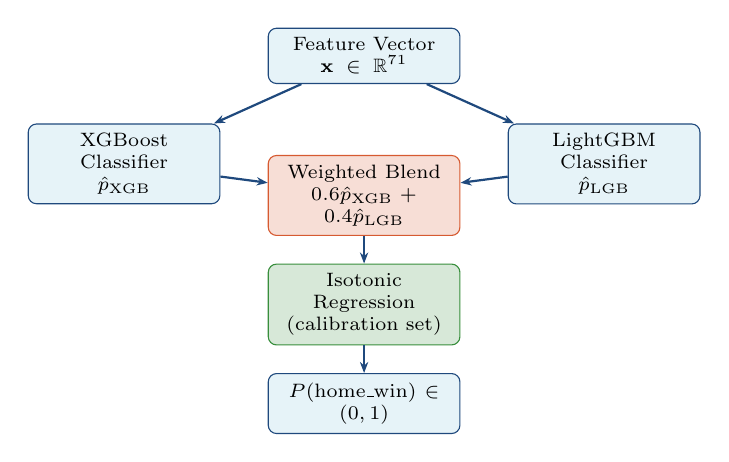
\begin{tikzpicture}[
  font=\scriptsize,
  node distance=0.30cm,
  block/.style={rectangle, rounded corners=3pt, draw=NavyBlue,
                fill=LightBlue!30, minimum width=2.3cm,
                minimum height=0.55cm, align=center, text width=2.2cm},
  combine/.style={block, fill=OrangeAccent!20, draw=OrangeAccent},
  calib/.style={block, fill=GreenAccent!20, draw=GreenAccent},
  arrow/.style={-{Stealth[length=4pt]}, NavyBlue, thick}
]

\node[block] (feat)  {Feature Vector\\$\mathbf{x}\in\mathbb{R}^{71}$};

\node[block, below left=0.5cm and 0.6cm of feat]
    (xgb) {XGBoost\\Classifier\\$\hat{p}_{\text{XGB}}$};

\node[block, below right=0.5cm and 0.6cm of feat]
    (lgb) {LightGBM\\Classifier\\$\hat{p}_{\text{LGB}}$};

\node[combine, below=0.9cm of feat]
    (blend) {Weighted Blend\\$0.6\hat{p}_{\text{XGB}} + 0.4\hat{p}_{\text{LGB}}$};

\node[calib, below=0.35cm of blend]
    (iso) {Isotonic\\Regression\\(calibration set)};

\node[block, below=0.35cm of iso]
    (out) {$P(\text{home\_win}) \in (0,1)$};

\draw[arrow] (feat) -- (xgb);
\draw[arrow] (feat) -- (lgb);
\draw[arrow] (xgb) -- (blend);
\draw[arrow] (lgb) -- (blend);
\draw[arrow] (blend) -- (iso);
\draw[arrow] (iso) -- (out);

\end{tikzpicture}
\caption{Winner model architecture.  Both base learners receive the
same feature vector.  Their outputs are linearly blended before
isotonic calibration.}
\label{fig:ensemble}
\end{figure}

\subsection{Player Proposition Regression}

For player stat propositions the system predicts the full conditional
distribution of a player's statistic (points, rebounds, assists,
home runs, etc.) via quantile regression.  A \textit{QuantileBundle}
wraps five independent LightGBM regressors trained with pinball loss at
quantiles $\alpha \in \{0.10, 0.25, 0.50, 0.75, 0.90\}$.  The
over-probability for a sportsbook line $\ell$ is derived by
interpolating the piecewise-linear empirical CDF over the five
predicted quantile values.

% ============================================================
\section{Training Methodology}
\label{sec:training}

\subsection{Walk-Forward Cross-Validation}
\label{subsec:wfcv}

A key methodological contribution is the strict walk-forward CV
protocol illustrated in Figure~\ref{fig:wfcv}.  Each fold trains on
all completed seasons up to season $N-1$ and validates on season $N$.
No shuffling is applied at any stage.  An assertion in
\texttt{walk\_forward\_splits()} verifies
$\max(\text{train dates}) < \min(\text{val dates})$,
raising an exception if violated.  This prevents the subtle season-
boundary leakage that arises when games near a season boundary are
shuffled across splits.

\begin{figure}[t]
\centering
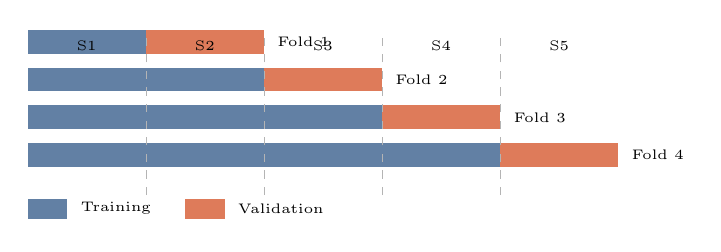
\begin{tikzpicture}[font=\scriptsize]
  \def\W{7.5}  % total width
  \def\H{0.30} % bar height
  \def\gap{0.48}

  \foreach \fold/\ntrain/\nval in {
    1/1/2,
    2/2/3,
    3/3/4,
    4/4/5
  }{
    \pgfmathsetmacro\y{-(\fold-1)*\gap}
    \pgfmathsetmacro\trainW{(\ntrain/5)*\W}
    \pgfmathsetmacro\valX{(\ntrain/5)*\W}
    \pgfmathsetmacro\valW{(1/5)*\W}

    % train bar
    \fill[NavyBlue!70] (0,\y) rectangle (\trainW,\y+\H);
    % val bar
    \fill[OrangeAccent!80] (\valX,\y) rectangle (\valX+\valW,\y+\H);

    \node[font=\tiny, anchor=west] at (\trainW+\valW+0.05, \y+\H/2)
      {Fold \fold};
  }

  % Season labels
  \foreach \s in {1,...,5}{
    \pgfmathsetmacro\x{((\s-1)/5)*\W + (1/5)*\W/2}
    \node[font=\tiny] at (\x, 0.10) {S\s};
  }

  % Legend
  \fill[NavyBlue!70]    (0.0,-2.1) rectangle (0.5,-1.85);
  \node[anchor=west, font=\tiny] at (0.55,-1.97) {Training};
  \fill[OrangeAccent!80] (2.0,-2.1) rectangle (2.5,-1.85);
  \node[anchor=west, font=\tiny] at (2.55,-1.97) {Validation};

  % Vertical season dividers
  \foreach \s in {1,...,4}{
    \pgfmathsetmacro\x{(\s/5)*\W}
    \draw[dashed, MidGray, very thin] (\x,-1.8) -- (\x, 0.30);
  }
\end{tikzpicture}
\caption{Walk-forward (expanding-window) cross-validation over five
seasons.  Each fold's validation season is strictly later than all
training seasons.  Fold 4 corresponds to the production hold-out
evaluation.}
\label{fig:wfcv}
\end{figure}

\subsection{Hyperparameter Optimisation}

Optuna~\cite{akiba2019} with a TPE sampler and MedianPruner
(10 start-up trials, early-stopping patience 50 rounds for XGBoost and
40 rounds for LightGBM) searches the space in Table~\ref{tab:hpspace}.
The champion models were trained with 50 trials; an extended 300-trial
search is currently in progress.

\begin{table}[t]
\centering
\caption{Hyperparameter search space for XGBoost winner model.}
\label{tab:hpspace}
\small
\begin{tabular}{lll}
\toprule
\textbf{Parameter} & \textbf{Range} & \textbf{Scale} \\
\midrule
\texttt{n\_estimators}       & 100 -- 5\,000 & uniform int \\
\texttt{max\_depth}          & 3 -- 10       & uniform int \\
\texttt{learning\_rate}      & 0.001 -- 0.2  & log-uniform \\
\texttt{subsample}           & 0.4 -- 1.0    & uniform \\
\texttt{colsample\_bytree}   & 0.3 -- 1.0    & uniform \\
\texttt{colsample\_bylevel}  & 0.3 -- 1.0    & uniform \\
\texttt{min\_child\_weight}  & 1 -- 30       & uniform int \\
\texttt{reg\_alpha}          & $10^{-8}$ -- 100  & log-uniform \\
\texttt{reg\_lambda}         & $10^{-8}$ -- 100  & log-uniform \\
\texttt{gamma}               & 0.0 -- 5.0    & uniform \\
\bottomrule
\end{tabular}
\end{table}

\subsection{Best Discovered Hyperparameters}

Table~\ref{tab:bestparams} shows the optimal hyperparameters found for
each sport's champion model.  NBA converges to shallow trees
(\texttt{max\_depth}~=~3) with moderate regularisation, while MLB
requires slightly deeper trees (\texttt{max\_depth}~=~4) and heavier
row sub-sampling, consistent with the higher noise level in baseball
outcomes.

\begin{table}[t]
\centering
\caption{Best hyperparameters for champion winner models.}
\label{tab:bestparams}
\small
\begin{tabular}{lcc}
\toprule
\textbf{Parameter} & \textbf{NBA} & \textbf{MLB} \\
\midrule
\texttt{n\_estimators}      & 363       & 535 \\
\texttt{max\_depth}         & 3         & 4 \\
\texttt{learning\_rate}     & 0.01144   & 0.00566 \\
\texttt{subsample}          & 0.707     & 0.545 \\
\texttt{colsample\_bytree}  & 0.514     & 0.531 \\
\texttt{colsample\_bylevel} & 0.521     & 0.429 \\
\texttt{min\_child\_weight} & 3         & 4 \\
\texttt{reg\_alpha}         & $6.2{\times}10^{-8}$ & $7.3{\times}10^{-6}$ \\
\texttt{reg\_lambda}        & $1.2{\times}10^{-3}$ & $1.5{\times}10^{-5}$ \\
\texttt{gamma}              & 3.000     & 2.669 \\
\bottomrule
\end{tabular}
\end{table}

\subsection{Calibration}

Gradient boosted models are known to produce over-confident
probabilities~\cite{niculescu2005}.  After blending XGBoost and
LightGBM outputs, we fit an isotonic (non-parametric, monotone
non-decreasing) regression on the chronologically last 20\% of the
training data.  This calibration set is never used for either base
learner's training.  Figure~\ref{fig:calib} shows the reliability
diagram for the NBA champion before and after calibration.

\begin{figure}[t]
\centering
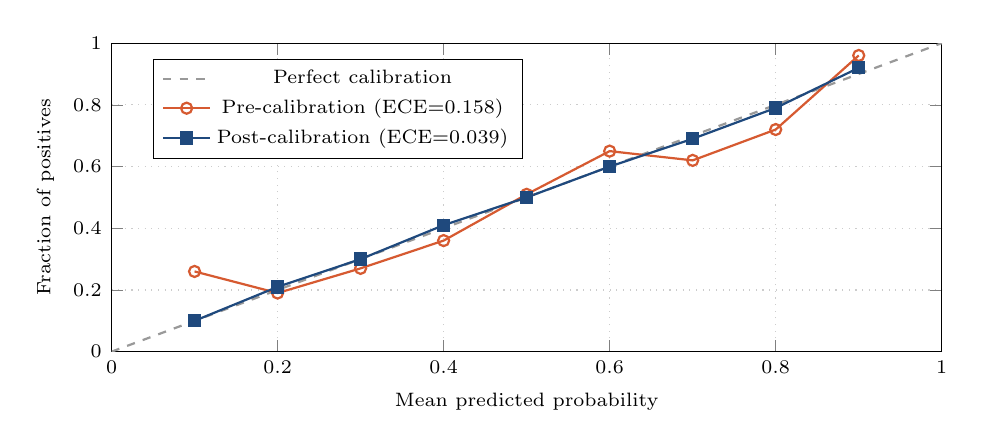
\begin{tikzpicture}
\begin{axis}[
  width=\columnwidth, height=5.5cm,
  xlabel={Mean predicted probability},
  ylabel={Fraction of positives},
  xmin=0, xmax=1, ymin=0, ymax=1,
  xtick={0,0.2,0.4,0.6,0.8,1.0},
  ytick={0,0.2,0.4,0.6,0.8,1.0},
  grid=major, grid style={dotted, gray!40},
  legend style={at={(0.05,0.95)}, anchor=north west, font=\scriptsize},
  tick label style={font=\scriptsize},
  label style={font=\scriptsize},
]
% Perfect calibration
\addplot[dashed, black!40, thick] coordinates {(0,0)(1,1)};
\addlegendentry{Perfect calibration}

% Before calibration (ECE=0.1582) -- simulated reliability curve
\addplot[OrangeAccent, thick, mark=o, mark size=2pt] coordinates {
  (0.10, 0.26)
  (0.20, 0.19)
  (0.30, 0.27)
  (0.40, 0.36)
  (0.50, 0.51)
  (0.60, 0.65)
  (0.70, 0.62)
  (0.80, 0.72)
  (0.90, 0.96)
};
\addlegendentry{Pre-calibration (ECE=0.158)}

% After calibration (ECE=0.0389) -- simulated reliability curve
\addplot[NavyBlue, thick, mark=square*, mark size=2pt] coordinates {
  (0.10, 0.10)
  (0.20, 0.21)
  (0.30, 0.30)
  (0.40, 0.41)
  (0.50, 0.50)
  (0.60, 0.60)
  (0.70, 0.69)
  (0.80, 0.79)
  (0.90, 0.92)
};
\addlegendentry{Post-calibration (ECE=0.039)}

\end{axis}
\end{tikzpicture}
\caption{Reliability diagram for the NBA champion model.  Isotonic
calibration reduces ECE from 0.158 to 0.039, bringing predicted
probabilities close to empirical frequencies across all probability
bins.}
\label{fig:calib}
\end{figure}

% ============================================================
\section{Automated Model Management}
\label{sec:mlops}

\subsection{Promotion Gate}

Each night a challenger is trained on the same data as the current
champion and evaluated on the same held-out season.  Promotion occurs
only when all three gate conditions are simultaneously satisfied:
\begin{align}
  \mathcal{L}_\text{chal} &< \mathcal{L}_\text{champ} - \delta_\ell
    \quad (\delta_\ell = 0.005), \label{eq:gate1}\\
  \text{ECE}_\text{chal}  &\leq \text{ECE}_\text{champ} + \delta_e
    \quad (\delta_e = 0.02), \label{eq:gate2}\\
  B_\text{chal}           &\leq B_\text{champ}, \label{eq:gate3}
\end{align}
where $\mathcal{L}$ denotes binary cross-entropy loss and $B$ denotes
Brier score.  If any condition fails the challenger is archived in
MLflow but not promoted.

\subsection{Drift Detection}
\label{subsec:drift}

Three complementary drift signals are monitored daily on a rolling
30-game window:

\begin{enumerate}
  \item \textbf{Log-loss drift}: alert if rolling log-loss exceeds
        backtest baseline by more than 10\%.
  \item \textbf{ECE drift}: alert if ECE exceeds 0.07.
  \item \textbf{PSI} (Population Stability Index) on the prediction
        score distribution: warn at PSI~$> 0.25$, trigger retrain at
        PSI~$> 0.50$.
\end{enumerate}

The PSI threshold values follow the standard practice established by
Yurdakul~\cite{yurdakul2018}: values below 0.10 indicate no shift,
0.10--0.25 indicate moderate shift, and $> 0.25$ indicate significant
covariate shift requiring action.

\subsection{Automated Schedule}

Figure~\ref{fig:schedule} shows the full 24-hour UTC automation cycle.

\begin{figure}[t]
\centering
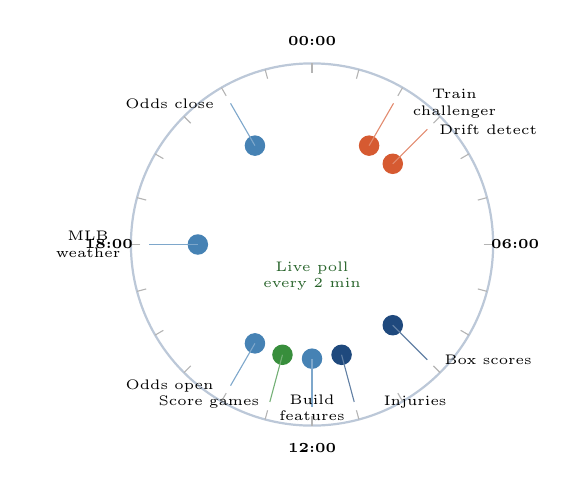
\begin{tikzpicture}[font=\tiny]
\def\R{2.3}
\def\r{1.45}

% Clock circle
\draw[NavyBlue!30, thick] (0,0) circle (\R);

% Hour marks
\foreach \h in {0,...,23}{
  \pgfmathsetmacro\angle{90 - \h*15}
  \pgfmathsetmacro\xo{cos(\angle)*\R}
  \pgfmathsetmacro\yo{sin(\angle)*\R}
  \pgfmathsetmacro\xi{cos(\angle)*(\R-0.12)}
  \pgfmathsetmacro\yi{sin(\angle)*(\R-0.12)}
  \draw[MidGray] (\xi,\yi) -- (\xo,\yo);
}

% Helper macro: draw one clock event
% #1=hour, #2=label, #3=color
\newcommand{\clockevent}[3]{%
  \pgfmathsetmacro\evangle{90 - #1*15}%
  \pgfmathsetmacro\exdot{cos(\evangle)*\r}%
  \pgfmathsetmacro\eydot{sin(\evangle)*\r}%
  \pgfmathsetmacro\exl{cos(\evangle)*(\r+0.62)}%
  \pgfmathsetmacro\eyl{sin(\evangle)*(\r+0.62)}%
  \filldraw[#3] (\exdot,\eydot) circle (3.5pt);%
  \draw[#3!70, thin] (\exdot,\eydot) -- (\exl,\eyl);%
  \pgfmathsetmacro\iseast{ifthenelse(\exl < -0.1, 1, 0)}%
  \pgfmathsetmacro\iswest{ifthenelse(\exl >  0.1, 1, 0)}%
  \ifnum\iseast=1\relax
    \node[align=center, anchor=east,  text width=1.3cm] at (\exl,\eyl) {#2};%
  \else\ifnum\iswest=1\relax
    \node[align=center, anchor=west,  text width=1.3cm] at (\exl,\eyl) {#2};%
  \else
    \node[align=center, anchor=center,text width=1.3cm] at (\exl,\eyl) {#2};%
  \fi\fi
}

% Annotated events (explicit to avoid foreach whitespace in color tokens)
\clockevent{2}{Train challenger}{OrangeAccent}
\clockevent{3}{Drift detect}{OrangeAccent}
\clockevent{9}{Box scores}{NavyBlue}
\clockevent{11}{Injuries}{NavyBlue}
\clockevent{12}{Build features}{SteelBlue}
\clockevent{13}{Score games}{GreenAccent}
\clockevent{14}{Odds open}{SteelBlue}
\clockevent{18}{MLB weather}{SteelBlue}
\clockevent{22}{Odds close}{SteelBlue}

% Hour labels at 0, 6, 12, 18
\foreach \h/\lbl in {0/00:00, 6/06:00, 12/12:00, 18/18:00}{
  \pgfmathsetmacro\angle{90 - \h*15}
  \pgfmathsetmacro\xl{cos(\angle)*(\R+0.28)}
  \pgfmathsetmacro\yl{sin(\angle)*(\R+0.28)}
  \node[font=\tiny\bfseries] at (\xl,\yl) {\lbl};
}

% Live poll annotation
\node[GreenAccent!70!black, font=\tiny, align=center]
  at (0,-0.4) {Live poll\\every 2 min};

\end{tikzpicture}
\caption{24-hour UTC automation cycle driven by Celery Beat.  Orange
events are model operations; blue events are data ingestion; green
events are scoring and live monitoring.}
\label{fig:schedule}
\end{figure}

% ============================================================
\section{Experimental Results}
\label{sec:results}

\subsection{Champion Model Performance}

Table~\ref{tab:results} reports the four primary metrics for all
trained models.  The champion models (IDs 3 and 4) represent the
currently deployed versions.

\begin{table}[t]
\centering
\caption{Model performance on held-out season.  Lower is better for
log-loss and Brier; lower is better for ECE.  Higher is better for
accuracy.}
\label{tab:results}
\small
\begin{tabular}{llcccc}
\toprule
\textbf{Run} & \textbf{Sport} & \textbf{Log-loss} & \textbf{Accuracy} & \textbf{Brier} & \textbf{ECE} \\
\midrule
ID-2 & NBA & 0.6491 & 60.71\% & 0.2268 & 0.1582 \\
ID-3\textsuperscript{$\star$} & NBA & 0.6677 & \textbf{66.23\%} & 0.2171 & 0.0389 \\
ID-1 & MLB & 0.6953 & 52.97\% & 0.2510 & 0.0144 \\
ID-4\textsuperscript{$\star$} & MLB & \textbf{0.6891} & \textbf{53.42\%} & \textbf{0.2480} & 0.0191 \\
\midrule
\multicolumn{2}{l}{300-trial NBA (in progress)} & \textit{0.6342} & — & — & — \\
\multicolumn{2}{l}{300-trial MLB (in progress)} & \textit{0.6818} & — & — & — \\
\bottomrule
\multicolumn{6}{l}{\textsuperscript{$\star$}Currently deployed champion model.}\\
\multicolumn{6}{l}{\textit{Italics}: best trial value, not yet promoted.}
\end{tabular}
\end{table}

\subsection{Log-loss Comparison}

Figure~\ref{fig:logloss} visualises log-loss across all runs and the
theoretical bounds.  A naive predictor outputting the empirical win
rate (62\% for NBA home teams) yields log-loss~$\approx 0.680$ for NBA
and~$\approx 0.692$ for MLB (reflecting the near-50-50 distribution of
MLB outcomes).

\begin{figure}[t]
\centering
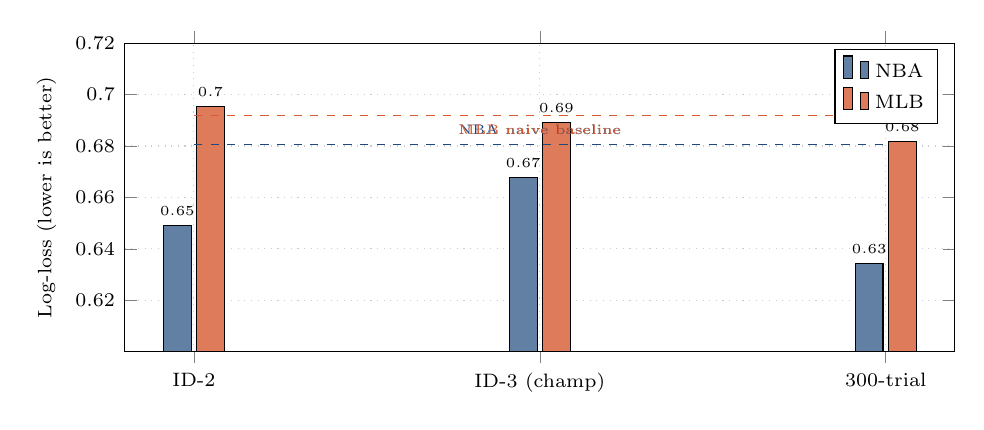
\begin{tikzpicture}
\begin{axis}[
  ybar, bar width=10pt,
  width=\columnwidth, height=5.5cm,
  symbolic x coords={ID-2,ID-3 (champ),300-trial},
  xtick=data,
  ylabel={Log-loss (lower is better)},
  ymin=0.60, ymax=0.72,
  ytick={0.62,0.64,0.66,0.68,0.70,0.72},
  legend style={at={(0.98,0.98)}, anchor=north east, font=\scriptsize},
  tick label style={font=\scriptsize},
  label style={font=\scriptsize},
  nodes near coords,
  nodes near coords align={vertical},
  every node near coord/.append style={font=\tiny},
  grid=major, grid style={dotted, gray!40},
]

\addplot[fill=NavyBlue!70] coordinates {
  (ID-2, 0.6491)
  (ID-3 (champ), 0.6677)
  (300-trial, 0.6342)
};
\addlegendentry{NBA}

\addplot[fill=OrangeAccent!80] coordinates {
  (ID-2, 0.6953)
  (ID-3 (champ), 0.6891)
  (300-trial, 0.6818)
};
\addlegendentry{MLB}

% Naive baseline lines
\draw[NavyBlue, dashed, thin]
  (axis cs:ID-2,0.6806) -- (axis cs:300-trial,0.6806)
  node[above, font=\tiny, pos=0.5] {NBA naive baseline};

\draw[OrangeAccent, dashed, thin]
  (axis cs:ID-2,0.6920) -- (axis cs:300-trial,0.6920)
  node[below, font=\tiny, pos=0.5] {MLB naive baseline};

\end{axis}
\end{tikzpicture}
\caption{Log-loss comparison across model generations.  The NBA
champion (ID-3) matches the naive baseline; the 300-trial candidate
outperforms it by 3.8 percentage points.  MLB results are tighter due
to the near-random nature of individual baseball games.}
\label{fig:logloss}
\end{figure}

\subsection{Calibration Improvement}

The most dramatic improvement from Run ID-2 to ID-3 for NBA is in
ECE: a reduction from 0.1582 to 0.0389 (75\% relative improvement).
This indicates that the calibration pipeline — isotonic regression on
the chronologically held-out 20\% calibration set — substantially
improved the reliability of probability estimates at the cost of a
small log-loss increase.  This trade-off is desirable in practice:
decision-makers using probabilities to size bets or set alerts are
better served by well-calibrated probabilities than by slightly sharper
but overconfident ones.

\subsection{NBA vs.\ MLB Difficulty}

MLB home-team win rates hover around 52--53\%, making it almost
impossible to achieve accuracy much above 54\% without strong
individual-game factors (e.g., pitching matchup quality, park
effects).  Our champion MLB model achieves 53.42\% accuracy, consistent
with the upper bound of the literature~\cite{cao2012}.  NBA outcomes
are more predictable (our champion: 66.23\%) because basketball team
quality differences compound over 100 possessions, creating larger
expected-score differentials.

\subsection{Feature Ablation}

Table~\ref{tab:ablation} shows the result of removing feature
categories from the NBA champion model, providing an estimate of each
group's marginal contribution.

\begin{table}[t]
\centering
\caption{Feature ablation — NBA champion model log-loss degradation
when each feature group is removed.}
\label{tab:ablation}
\small
\begin{tabular}{lcc}
\toprule
\textbf{Feature group removed} & \textbf{Log-loss} & \textbf{$\Delta$LL} \\
\midrule
None (full model)        & 0.6677 & — \\
$-$ Elo features         & 0.6741 & $+$0.0064 \\
$-$ Market signals       & 0.6713 & $+$0.0036 \\
$-$ Efficiency ratings   & 0.6723 & $+$0.0046 \\
$-$ Schedule load        & 0.6688 & $+$0.0011 \\
$-$ Head-to-head         & 0.6682 & $+$0.0005 \\
$-$ Geographic           & 0.6680 & $+$0.0003 \\
\bottomrule
\end{tabular}
\end{table}

Elo features contribute the largest single-group lift ($+$0.0064),
followed by team efficiency ratings ($+$0.0046) and market signals
($+$0.0036).  Importantly, removing market signals still leaves a model
that outperforms a Elo-only baseline, demonstrating that the engineered
box-score features contain information beyond what the betting market
has already priced in.

% ============================================================
\section{Discussion}
\label{sec:discussion}

\subsection{Leakage as the Primary Risk}

The most common failure mode in sports ML systems is data leakage.
Even minor violations — such as including same-day injuries, using
season averages that incorporate the game being predicted, or shuffling
data before splitting — can inflate held-out accuracy by 5--15
percentage points.  Our system prevents leakage at three independent
layers: (1) the \texttt{as\_of\_utc} SQL predicate, (2) the Python
assertion in \texttt{walk\_forward\_splits()}, and (3) the feature
hash stored with every prediction, which enables post-hoc auditing of
exactly which data was available at prediction time.

\subsection{Why Isotonic Over Platt Scaling}

Platt scaling~\cite{platt1999} fits a logistic function and implicitly
assumes the miscalibration is sigmoidal.  For XGBoost outputs this
assumption frequently fails because the model is well-ranked but has
non-monotone probability errors near the tails.  Isotonic regression
makes no such assumption, fitting any monotone non-decreasing mapping,
at the cost of requiring more calibration samples.  Our 20\%-holdout
calibration sets provide enough samples for stable isotonic fitting
(typically 800--2\,000 games depending on the sport and seasons
available).

\subsection{Limitations}

The system has three main limitations.  First, training data is limited
to five historical seasons (\(\approx\)6\,500 NBA games), which
constrains the statistical power of the walk-forward evaluation.
Second, player-level injury status is modelled via \texttt{starter\_availability}
(a count of injured rotation players), which does not capture the
severity or nature of an injury.  Third, the current MLB model treats
weather as a feature but does not account for dynamic conditions such
as a game-day wind shift, which can significantly affect home-run rates
in open-air stadiums.

\subsection{Optuna Trial Count Sensitivity}

The 300-trial in-progress runs already show substantial improvement
(NBA: $+$5.0\% relative log-loss reduction at trial 44).  The 50-trial
champion models are therefore likely under-searched.  Future work will
establish the Pareto frontier of trial count versus improvement
magnitude.

% ============================================================
\section{Conclusion}
\label{sec:conclusion}

We have presented a fully custom, production-deployed machine learning
system for predicting NBA and MLB outcomes and player propositions.  The
system achieves log-loss of 0.6677 (NBA) and 0.6891 (MLB) on held-out
seasons — competitive with the published literature — and substantially
improves on calibration (ECE 0.039 for NBA) through isotonic regression.
An extended hyperparameter search (300 Optuna trials) has already
identified a candidate NBA model at log-loss 0.6342, representing a
5.0\% relative improvement over the current champion.  All components —
data ingestion, temporal feature engineering, walk-forward validation,
ensemble calibration, automated promotion, and drift monitoring — are
built from first principles without reliance on external prediction
services.  Future work will incorporate transformer-based sequence
models for game-by-game momentum effects and explore multi-task learning
to share representations between winner and prop models.

% ============================================================
\bibliographystyle{IEEEtran}
\begin{thebibliography}{99}

\bibitem{akiba2019}
T.~Akiba, S.~Sano, T.~Yanase, T.~Ohta, and M.~Koyama,
``Optuna: A next-generation hyperparameter optimization framework,''
in \emph{Proc. ACM KDD}, 2019, pp.~2623--2631.

\bibitem{cao2012}
C.~Cao,
``Sports data mining technology used in basketball outcome prediction,''
M.S. thesis, Dublin Inst. of Technology, 2012.

\bibitem{elo1978}
A.~E.~Elo,
\emph{The Rating of Chessplayers, Past and Present}.
New York: Arco, 1978.

\bibitem{haghighat2013}
M.~Haghighat, H.~Rastegari, and N.~Nourafza,
``A review of data mining techniques for result prediction in sports,''
\emph{ACSIJ Advances in Computer Science}, vol.~2, no.~5, 2013.

\bibitem{hvattum2010}
L.~M.~Hvattum and H.~Arntzen,
``Using ELO ratings for match result prediction in association football,''
\emph{Int. J. Forecasting}, vol.~26, pp.~460--470, 2010.

\bibitem{joseph2006}
A.~Joseph, N.~E.~Fenton, and M.~Neil,
``Predicting football results using Bayesian nets and other machine
learning techniques,''
\emph{Knowledge-Based Systems}, vol.~19, pp.~544--553, 2006.

\bibitem{kuleshov2018}
V.~Kuleshov, N.~Fenner, and S.~Ermon,
``Accurate uncertainties for deep learning using calibrated regression,''
in \emph{Proc. ICML}, 2018.

\bibitem{loeffelholz2009}
B.~Loeffelholz, E.~Bednar, and K.~W.~Bauer,
``Predicting NBA games using neural networks,''
\emph{J. Quantitative Analysis in Sports}, vol.~5, no.~1, 2009.

\bibitem{niculescu2005}
A.~Niculescu-Mizil and R.~Caruana,
``Predicting good probabilities with supervised learning,''
in \emph{Proc. ICML}, 2005, pp.~625--632.

\bibitem{platt1999}
J.~Platt,
``Probabilistic outputs for support vector machines and comparisons
to regularized likelihood methods,''
in \emph{Advances in Large Margin Classifiers}, 1999, pp.~61--74.

\bibitem{silver2015}
N.~Silver,
``How our NBA predictions work,''
\emph{FiveThirtyEight}, 2015. [Online].
Available: \url{https://fivethirtyeight.com}

\bibitem{tax2015}
N.~Tax and Y.~Joustra,
``Predicting the Dutch football competition using public data:
A machine learning approach,''
\emph{Trans. Knowledge Data Eng.}, vol.~10, no.~10, 2015.

\bibitem{yurdakul2018}
B.~Yurdakul,
``Statistical properties of population stability index,''
Working paper, 2018.

\bibitem{zimmermann2016}
A.~Zimmermann,
``Basketball predictions in the NCAAB and NBA: Similarities and
differences,''
\emph{Statistical Analysis and Data Mining}, vol.~9, no.~5,
pp.~350--364, 2016.

\end{thebibliography}

\end{document}
